\section{7 Sep 23 - Activity: Numerical Integration and More
Lagrangians}\label{sep-23---activity-numerical-integration-and-more-lagrangians}

Now that we have an idea how to find a wealth of interesting ordinary
differential equations using Lagrangian mechanics, we'll work on
building up ways to understand these equations, their solutions and
behavior. The issue with this is that \textbf{most ODEs do not have
analytical solutions}. That means we can't write down nice closed-form
solutions for them using transcendental functions. However, don't
despair, because that does not mean there is no solution. In fact, the
vast majority of non-pathological ODEs one might come across in physics
are \textbf{guaranteed} to have unique solutions (at least for finite
time). We can easily calculate these solutions using \textbf{numerical
integration}. Next week we'll also see how we can characterize the
behavior of ODEs even without access to numerical integration.

\subsection{The Simple Harmonic
Oscillator}\label{the-simple-harmonic-oscillator}

Let's start simple with everyone's favorite differential equation, the
simple harmonic oscillator. Recall that we can write the SHO as:

\[
\ddot{x} =  -\omega_0^2x
\]

where \(\omega_0^2 = \frac{k}{m}\). This equation is 2nd order, but
numerical integration techniques only work on 1st order equations.
Thankfully they work on any number of potentially coupled 1st order
equations. This means that with a quick change of variables, we can
write the SHO as a system of 2 first order equations by introducing a
new variable \(v\) equal to the velocity of the oscillator.

\[
v = \dot{x}
\]

Then the acceleration of the oscillator can be written as:

\[
\dot{v}  = -\omega_0^2x
\]

This trick for writing higher order differential equations as first
order equations is incredibly common.

\subsubsection{Setting up to numerically
integrate}\label{setting-up-to-numerically-integrate}

We need a few things to numerically integrate using \texttt{solve\_ivp}
in python. First, we import the relevant libraries and functions.

\begin{Shaded}
\begin{Highlighting}[]
\CommentTok{\# Import libraries}
\ImportTok{import}\NormalTok{ matplotlib.pyplot }\ImportTok{as}\NormalTok{ plt}
\ImportTok{import}\NormalTok{ numpy }\ImportTok{as}\NormalTok{ np}
\ImportTok{import}\NormalTok{ matplotlib.pyplot }\ImportTok{as}\NormalTok{ plt}
\ImportTok{from}\NormalTok{ scipy.integrate }\ImportTok{import}\NormalTok{ solve\_ivp}
\end{Highlighting}
\end{Shaded}

**Note: The code in this block is not meant to be run directly, it is
just a reference for the steps we need to take. Working code that is put
together appears in the next cell.*

\paragraph{1. Derivatives Function}\label{derivatives-function}

First, we need to set up a derivatives function that calculates and
returns a list of the values of the first order derivatives given an
input list of current values. These current values represent a location
in \textbf{phase space}. As we will learn,
\href{https://en.wikipedia.org/wiki/Phase_space}{phase space} is a space
that contains all the information about the state of an ODE. The simple
harmonic oscillator has a 2D phase space since its state is totally
defined by its position and velocity.

Here's what our derivatives function looks like for a SHO:

\begin{Shaded}
\begin{Highlighting}[]
\KeywordTok{def}\NormalTok{ diffyqs(t, curr\_vals, omega2):}
    \CommentTok{\# 2 first{-}order differential equations for a SHO}
    \CommentTok{\# first 2 arguments are always t and curr\_vals, which are followed by any parameters of your ODEs}
\NormalTok{    x, v }\OperatorTok{=}\NormalTok{ curr\_vals   }\CommentTok{\# unpack current values}
    
\NormalTok{    vdot }\OperatorTok{=} \OperatorTok{{-}}\NormalTok{omega2 }\OperatorTok{*}\NormalTok{ x }\CommentTok{\# calculate derivative}

    \ControlFlowTok{return}\NormalTok{ v, vdot }\CommentTok{\# return derivatives}
\end{Highlighting}
\end{Shaded}

We will pass this function to our solver, which will give us back
integrated solutions of our list of derivatives. So since
\(v = \dot{x}\), our solution will return \(x\) first, and \(v\).

\paragraph{2. Time Setup}\label{time-setup}

We need to define the time span to solve the ODE for AND the specific
times we'd like solution points for. Here it is also convienient to
choose a time step \(dt\). Here's one way we could do this in python:

\begin{Shaded}
\begin{Highlighting}[]
\NormalTok{tmax }\OperatorTok{=} \DecValTok{15}
\NormalTok{dt }\OperatorTok{=} \FloatTok{0.1}
\NormalTok{tspan }\OperatorTok{=}\NormalTok{ (}\DecValTok{0}\NormalTok{, tmax)         }\CommentTok{\# time span}
\NormalTok{t }\OperatorTok{=}\NormalTok{ np.arange(}\DecValTok{0}\NormalTok{, tmax, dt) }\CommentTok{\# specific times to return solutions for}
\end{Highlighting}
\end{Shaded}

\paragraph{3. Parameters and Initial
Conditions}\label{parameters-and-initial-conditions}

Since we're dealing with ODEs, we need to supply an initial condition to
be able to solve. The SHO has 2D phase space so we need 2 values for our
initial condition. We'll also define parameter value(s) in this step.

\begin{Shaded}
\begin{Highlighting}[]
\NormalTok{omega2 }\OperatorTok{=} \DecValTok{2}
\NormalTok{initial\_condition }\OperatorTok{=}\NormalTok{ [}\DecValTok{1}\NormalTok{, }\DecValTok{0}\NormalTok{] }\CommentTok{\# pull back 1m, no initial velocity}
\end{Highlighting}
\end{Shaded}

\paragraph{4. Call Integrator}\label{call-integrator}

Now all we have left to do is to actually use \texttt{solve\_ivp} to do
the integration. The syntax for how to do this is shown below. We also
get the opportunity to tell \texttt{solve\_ivp} exactly what numerical
integration method we'd like it to use. For now we can think of the
integrator as a magic box and choose \texttt{RK45}, or a Runge-Kutta 4th
order method.

\begin{Shaded}
\begin{Highlighting}[]
\NormalTok{solved }\OperatorTok{=}\NormalTok{ solve\_ivp(diffyqs, tspan, initial\_condition, t\_eval }\OperatorTok{=}\NormalTok{ t, args }\OperatorTok{=}\NormalTok{ (omega2, ), method}\OperatorTok{=}\StringTok{"RK45"}\NormalTok{)}
\end{Highlighting}
\end{Shaded}

To access the solution directly, use \texttt{solved.y}. The variable
\texttt{solved.y{[}0{]}} is the solved for position array and
\texttt{solved.y{[}1{]}} is the velocity array in this case. Now let's
see a full implementation of this below, including some visualization
that compares our numerical solution to the analytical solution of the
SHO.

\begin{Shaded}
\begin{Highlighting}[]
\CommentTok{\# 1. Derivatives Function}
\KeywordTok{def}\NormalTok{ diffyqs(t, curr\_vals, omega2):}
\NormalTok{    x, v }\OperatorTok{=}\NormalTok{ curr\_vals }
\NormalTok{    vdot }\OperatorTok{=} \OperatorTok{{-}}\NormalTok{omega2 }\OperatorTok{*}\NormalTok{ x}
    \ControlFlowTok{return}\NormalTok{ v, vdot}

\CommentTok{\# 2. Time Setup}
\NormalTok{tmax }\OperatorTok{=} \DecValTok{50}
\NormalTok{dt }\OperatorTok{=} \FloatTok{0.1}
\NormalTok{tspan }\OperatorTok{=}\NormalTok{ (}\DecValTok{0}\NormalTok{, tmax)}
\NormalTok{t }\OperatorTok{=}\NormalTok{ np.arange(}\DecValTok{0}\NormalTok{, tmax, dt)}

\CommentTok{\# 3. Parameters and Initial Conditions}
\NormalTok{omega2 }\OperatorTok{=} \DecValTok{2}
\NormalTok{initial\_condition }\OperatorTok{=}\NormalTok{ [}\DecValTok{1}\NormalTok{, }\DecValTok{0}\NormalTok{] }

\CommentTok{\# 4. Call Integrator (note we can swamp them out, RK45 is the default)}
\NormalTok{RK23solved }\OperatorTok{=}\NormalTok{ solve\_ivp(diffyqs, tspan, initial\_condition, t\_eval }\OperatorTok{=}\NormalTok{ t, args }\OperatorTok{=}\NormalTok{ (omega2,), method}\OperatorTok{=}\StringTok{"RK23"}\NormalTok{)}
\NormalTok{RK45solved }\OperatorTok{=}\NormalTok{ solve\_ivp(diffyqs, tspan, initial\_condition, t\_eval }\OperatorTok{=}\NormalTok{ t, args }\OperatorTok{=}\NormalTok{ (omega2,), method}\OperatorTok{=}\StringTok{"RK45"}\NormalTok{)}

\CommentTok{\# 5. Visualization and Comparison to analytical solution}
\KeywordTok{def}\NormalTok{ analytic\_sol(t, omega0, initial\_condition):}
\NormalTok{    x0, v0 }\OperatorTok{=}\NormalTok{ initial\_condition}
    \ControlFlowTok{return}\NormalTok{ (v0}\OperatorTok{/}\NormalTok{omega0)}\OperatorTok{*}\NormalTok{np.sin(omega0}\OperatorTok{*}\NormalTok{t) }\OperatorTok{+}\NormalTok{ x0 }\OperatorTok{*}\NormalTok{ np.cos(omega0}\OperatorTok{*}\NormalTok{t)}

\NormalTok{plt.figure(figsize}\OperatorTok{=}\NormalTok{(}\DecValTok{16}\NormalTok{, }\DecValTok{4}\NormalTok{))}
\NormalTok{plt.plot(t, analytic\_sol(t, omega2}\OperatorTok{**}\FloatTok{0.5}\NormalTok{,initial\_condition), label }\OperatorTok{=} \StringTok{"Analytic Solution"}\NormalTok{, linewidth }\OperatorTok{=} \DecValTok{3}\NormalTok{)}
\NormalTok{plt.plot(t, RK23solved.y[}\DecValTok{0}\NormalTok{], label }\OperatorTok{=} \StringTok{"Numerical Solution (RK23)"}\NormalTok{, marker}\OperatorTok{=}\StringTok{\textquotesingle{}*\textquotesingle{}}\NormalTok{)}
\NormalTok{plt.title(}\StringTok{"Long term SHO motion with RK23 solution"}\NormalTok{)}
\NormalTok{plt.xlabel(}\StringTok{"t"}\NormalTok{)}
\NormalTok{plt.ylabel(}\StringTok{"x"}\NormalTok{)}
\NormalTok{plt.legend()}
\NormalTok{plt.grid()}

\NormalTok{plt.figure(figsize}\OperatorTok{=}\NormalTok{(}\DecValTok{16}\NormalTok{,}\DecValTok{4}\NormalTok{))}
\NormalTok{plt.plot(t,analytic\_sol(t, omega2}\OperatorTok{**}\FloatTok{0.5}\NormalTok{,initial\_condition), label }\OperatorTok{=} \StringTok{"Analytic Solution"}\NormalTok{, linewidth }\OperatorTok{=} \DecValTok{3}\NormalTok{)}
\NormalTok{plt.plot(t,RK45solved.y[}\DecValTok{0}\NormalTok{], label }\OperatorTok{=} \StringTok{"Numerical Solution (RK45"}\NormalTok{, marker}\OperatorTok{=}\StringTok{\textquotesingle{}s\textquotesingle{}}\NormalTok{)}
\NormalTok{plt.title(}\StringTok{"Long term SHO motion with RK45 solution"}\NormalTok{)}
\NormalTok{plt.xlabel(}\StringTok{"t"}\NormalTok{)}
\NormalTok{plt.ylabel(}\StringTok{"x"}\NormalTok{)}
\NormalTok{plt.legend()}
\NormalTok{plt.grid()}
\end{Highlighting}
\end{Shaded}

\begin{figure}
\centering
\pandocbounded{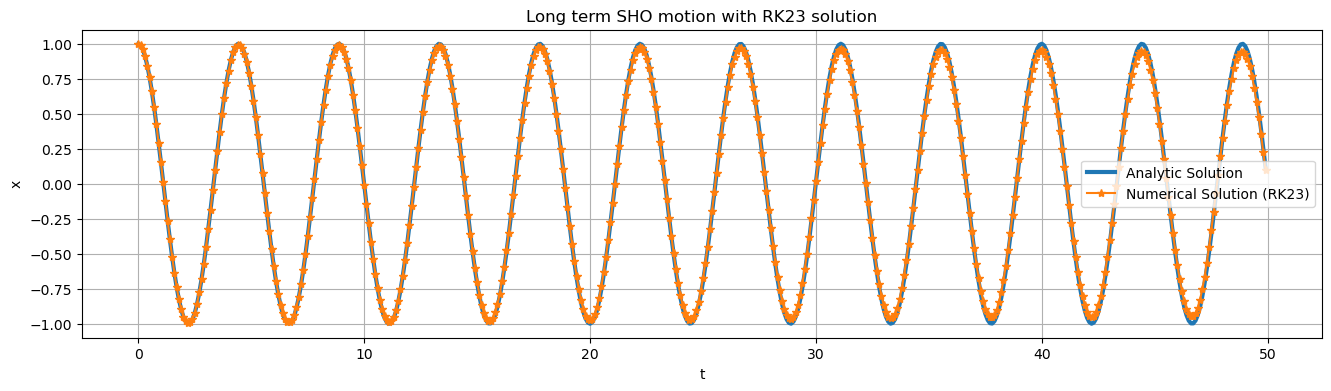
\includegraphics[keepaspectratio,alt={png}]{../images/activity-lagrange_2_activity-lagrange_2_tmp_4_0.png}}
\caption{png}
\end{figure}

\begin{figure}
\centering
\pandocbounded{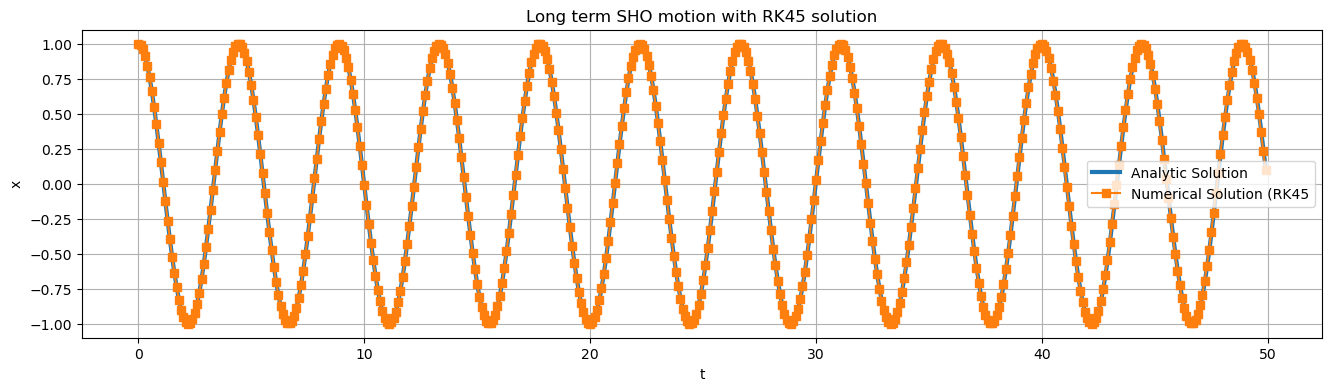
\includegraphics[keepaspectratio,alt={png}]{../images/activity-lagrange_2_activity-lagrange_2_tmp_4_1.png}}
\caption{png}
\end{figure}

\subsection{Group Activity}\label{group-activity}

\subsubsection{Back to Paraboloid
Paradise}\label{back-to-paraboloid-paradise}

\href{../../assets/notes/Notes-Bead_in_a_Paraboloid.pdf}{Analytical
Solution (Finding ODEs for Paraboloid)}

Let's consider the problem where a particle was constrained to move on
the surface \(z = c\rho^2\). The EOM we arrived at are complex
\[\ddot{\rho} = \dfrac{\rho\dot{\phi}^2 - 4c^2\rho\dot{\rho}^2 -2cg\rho}{1 + 4c^2\rho^2}\]
\[\ddot{\phi} = -2\frac{\dot{\rho}\dot{\phi}}{\rho} \]

\textbf{✅ Do this}

Introduce variables \(v\) and \(\omega\) to use our trick for reducing
\(>1\) order differential equations to first order equations to write
the equations of motion for this problem as a system of four first order
differential equations (shown below). \textbf{You may set c=1, but keep
it as a variable.}

\[\dot{\rho} = ?? \]

\[\dot{v} = ??\]

\[\dot{\phi} = ?? \]

\[\dot{\omega} = ??\]

\textbf{✅ Do this}

Use these equations to correct the \texttt{diffyqs} function in the cell
below.

\begin{Shaded}
\begin{Highlighting}[]
\CommentTok{\# 1. Derivatives Function}
\KeywordTok{def}\NormalTok{ diffyqs(t, curr\_vals, g, c):}

\NormalTok{    r, v, theta, omega }\OperatorTok{=}\NormalTok{ curr\_vals}
    
\NormalTok{    vdot }\OperatorTok{=} \DecValTok{0}

\NormalTok{    omegadot }\OperatorTok{=} \DecValTok{0}

    \ControlFlowTok{return}\NormalTok{ v, vdot, omega, omegadot }\CommentTok{\# solution will return in this order, but integrated (r,v,theta,ω)}

\CommentTok{\# 2. Time Setup}
\NormalTok{tmax }\OperatorTok{=} \DecValTok{40}
\NormalTok{dt }\OperatorTok{=} \FloatTok{0.01} \CommentTok{\# unneccecarily small dt to make plot super smooth}
\NormalTok{t }\OperatorTok{=}\NormalTok{ np.arange(}\DecValTok{0}\NormalTok{, tmax, dt)}

\CommentTok{\# 3. Parameters and Initial Conditions}
\NormalTok{c }\OperatorTok{=} \DecValTok{1}
\NormalTok{g }\OperatorTok{=} \FloatTok{9.81}
\NormalTok{x0 }\OperatorTok{=}\NormalTok{ [}\FloatTok{2.6}\NormalTok{,}\DecValTok{0}\NormalTok{,}\DecValTok{0}\NormalTok{,}\DecValTok{2}\NormalTok{] }

\CommentTok{\# 4. Call Integrator}
\NormalTok{solved }\OperatorTok{=}\NormalTok{ solve\_ivp(diffyqs, (}\DecValTok{0}\NormalTok{, tmax), x0, t\_eval }\OperatorTok{=}\NormalTok{ t, args }\OperatorTok{=}\NormalTok{ (g, c, ), method}\OperatorTok{=}\StringTok{"RK45"}\NormalTok{)}
\end{Highlighting}
\end{Shaded}

\textbf{✅ Do this}

\begin{enumerate}
\def\labelenumi{\arabic{enumi}.}
\item
  Make r vs t and theta vs t plots of this trajectory. Can you think of
  what that trajectory would look like in cartesian coordinates? 2. Run
  the cell below to see what the trajectory looks like in 3D. How does
  the true trajectory compare to your prediction?
\item
  Change the initial condtion to examine the following cases and plot
  the trajectories in 3d:

  \begin{enumerate}
  \def\labelenumii{\alph{enumii}.}
  \item
    Particle starts from rest and is let go
  \item
    Particle starts at a given height and is given a low speed (less
    than needed to orbit)
  \item
    Particle starts at a given height and is given a low speed (more
    than needed to orbit)
  \item
    Can you find a flat horizontal circular orbit?
  \end{enumerate}
\end{enumerate}

\begin{Shaded}
\begin{Highlighting}[]
\KeywordTok{def}\NormalTok{ parabaloid(x, y, alpha}\OperatorTok{=}\FloatTok{1.}\NormalTok{):}
    \CommentTok{\# function of a paraboloid in Cartesian coordinates}
    \ControlFlowTok{return}\NormalTok{ alpha }\OperatorTok{*}\NormalTok{ (x}\OperatorTok{**}\DecValTok{2} \OperatorTok{+}\NormalTok{ y}\OperatorTok{**}\DecValTok{2}\NormalTok{)}

\KeywordTok{def}\NormalTok{ cylindrical\_to\_cartesian(r, th, alpha}\OperatorTok{=}\FloatTok{1.}\NormalTok{):}
    \CommentTok{\# convert back to cartesian coordinates for ease of plotting}
\NormalTok{    r }\OperatorTok{=}\NormalTok{ np.array(r)}
\NormalTok{    th }\OperatorTok{=}\NormalTok{ np.array(th)}
\NormalTok{    x }\OperatorTok{=}\NormalTok{ r}\OperatorTok{*}\NormalTok{np.cos(th)}
\NormalTok{    y }\OperatorTok{=}\NormalTok{ r}\OperatorTok{*}\NormalTok{np.sin(th)}
    \ControlFlowTok{return}\NormalTok{ x,y,parabaloid(x, y, alpha)}

\KeywordTok{def}\NormalTok{ plot\_solution(solved):}
    \CommentTok{\# Function to plot the trajectory }

    \CommentTok{\# points of the surface to plot}
\NormalTok{    x }\OperatorTok{=}\NormalTok{ np.linspace(}\OperatorTok{{-}}\FloatTok{2.8}\NormalTok{, }\FloatTok{2.8}\NormalTok{, }\DecValTok{50}\NormalTok{)}
\NormalTok{    y }\OperatorTok{=}\NormalTok{ np.linspace(}\OperatorTok{{-}}\FloatTok{2.8}\NormalTok{, }\FloatTok{2.8}\NormalTok{, }\DecValTok{50}\NormalTok{)}
\NormalTok{    alpha }\OperatorTok{=}\NormalTok{ c}
    \CommentTok{\# construct meshgrid for plotting}
\NormalTok{    X, Y }\OperatorTok{=}\NormalTok{ np.meshgrid(x, y)}
\NormalTok{    Z }\OperatorTok{=}\NormalTok{ parabaloid(X, Y, alpha)}

    \CommentTok{\# get trajectory in cartesian coords}
\NormalTok{    xtraj, ytraj, ztraj }\OperatorTok{=}\NormalTok{ cylindrical\_to\_cartesian(solved.y[}\DecValTok{0}\NormalTok{], solved.y[}\DecValTok{2}\NormalTok{], alpha)}

    \CommentTok{\# plot plot plot}
\NormalTok{    fig }\OperatorTok{=}\NormalTok{ plt.figure(figsize }\OperatorTok{=}\NormalTok{ (}\DecValTok{10}\NormalTok{,}\DecValTok{10}\NormalTok{))}
\NormalTok{    ax }\OperatorTok{=}\NormalTok{ plt.axes(projection}\OperatorTok{=}\StringTok{\textquotesingle{}3d\textquotesingle{}}\NormalTok{)}
\NormalTok{    plt.title(}\StringTok{"Particle\textquotesingle{}s Path in 3d"}\NormalTok{)}
\NormalTok{    ax.plot\_surface(X, Y, Z, cmap}\OperatorTok{=}\StringTok{\textquotesingle{}binary\textquotesingle{}}\NormalTok{, alpha}\OperatorTok{=}\FloatTok{0.5}\NormalTok{) }
\NormalTok{    ax.plot3D(xtraj, ytraj, ztraj, c }\OperatorTok{=} \StringTok{"\#18453B"}\NormalTok{)}
\NormalTok{    ax.set\_xlim(}\OperatorTok{{-}}\DecValTok{3}\NormalTok{, }\DecValTok{3}\NormalTok{)}\OperatorTok{;}\NormalTok{ ax.set\_ylim(}\OperatorTok{{-}}\DecValTok{3}\NormalTok{, }\DecValTok{3}\NormalTok{)}\OperatorTok{;}\NormalTok{ ax.set\_zlim(}\OperatorTok{{-}}\DecValTok{1}\NormalTok{ ,}\DecValTok{15}\NormalTok{)}
\NormalTok{    ax.set\_xlabel(}\StringTok{\textquotesingle{}x\textquotesingle{}}\NormalTok{)}
\NormalTok{    ax.set\_ylabel(}\StringTok{\textquotesingle{}y\textquotesingle{}}\NormalTok{)}
\NormalTok{    ax.set\_zlabel(}\StringTok{\textquotesingle{}z\textquotesingle{}}\NormalTok{)}
\NormalTok{    plt.show()}

\NormalTok{plot\_solution(solved)}
\end{Highlighting}
\end{Shaded}

\begin{figure}
\centering
\pandocbounded{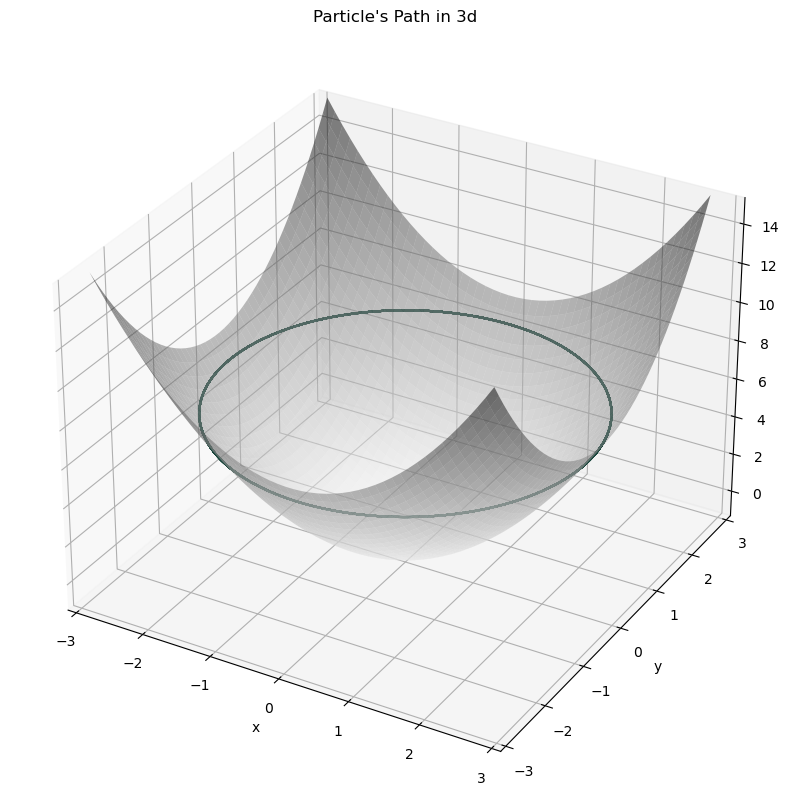
\includegraphics[keepaspectratio,alt={png}]{../images/activity-lagrange_2_activity-lagrange_2_tmp_8_0.png}}
\caption{png}
\end{figure}

\begin{Shaded}
\begin{Highlighting}[]

\end{Highlighting}
\end{Shaded}
